\documentclass[12pt]{article}

%%%%%%%%%%%%%%%%%%%%%%%%%%%%%%%%%%%%%%%%%%%%%%%%%%%%%%%%%%%%%%%%%%%%%%%%%%%%%%%%%%%%%%%%%%%%%%%%%%%%
% Math
\usepackage{fancyhdr} 
\usepackage{amsfonts}
\usepackage{amsmath}
\usepackage{amssymb}
\usepackage{amsthm}
\usepackage{enumitem}
%\usepackage{dsfont}

%%%%%%%%%%%%%%%%%%%%%%%%%%%%%%%%%%%%%%%%%%%%%%%%%%%%%%%%%%%%%%%%%%%%%%%%%%%%%%%%%%%%%%%%%%%%%%%%%%%%
% Macros
\usepackage{calc}

%%%%%%%%%%%%%%%%%%%%%%%%%%%%%%%%%%%%%%%%%%%%%%%%%%%%%%%%%%%%%%%%%%%%%%%%%%%%%%%%%%%%%%%%%%%%%%%%%%%%
% Commands and Custom Variables	
\newcommand{\problem}[1]{\hspace{-4 ex} \large \textbf{Problem #1} }
\let\oldemptyset\emptyset
\let\emptyset\varnothing
\newcommand{\norm}[1]{\left\lVert#1\right\rVert}
\newcommand{\sint}{\text{s}\kern-5pt\int}
\newcommand{\powerset}{\mathcal{P}}
\renewenvironment{proof}{\hspace{-4 ex} \emph{Proof}:}{\qed}
\newcommand{\RR}{\mathbb{R}}
\newcommand{\NN}{\mathbb{N}}
\newcommand{\QQ}{\mathbb{Q}}
\newcommand{\ZZ}{\mathbb{Z}}
\newcommand{\CC}{\mathbb{C}}
\renewcommand{\Re}{\operatorname{Re}}
\renewcommand{\Im}{\operatorname{Im}}

\newcommand{\solution}{\vspace{2 ex} \hspace{-5 ex} \emph{Solution.} }


%%%%%%%%%%%%%%%%%%%%%%%%%%%%%%%%%%%%%%%%%%%%%%%%%%%%%%%%%%%%%%%%%%%%%%%%%%%%%%%%%%%%%%%%%%%%%%%%%%%%
%page
\usepackage[margin=1in]{geometry}
\usepackage{setspace}
%\doublespacing
\allowdisplaybreaks
\pagestyle{fancy}
\fancyhf{}
\rhead{Malmuth \& Shaw \space \thepage}
\setlength\parindent{0pt}

%%%%%%%%%%%%%%%%%%%%%%%%%%%%%%%%%%%%%%%%%%%%%%%%%%%%%%%%%%%%%%%%%%%%%%%%%%%%%%%%%%%%%%%%%%%%%%%%%%%%
%Code
\usepackage{listings}
\usepackage{courier}
\lstset{
	language=Python,
	showstringspaces=false,
	formfeed=newpage,
	tabsize=4,
	commentstyle=\itshape,
	basicstyle=\ttfamily,
}

%%%%%%%%%%%%%%%%%%%%%%%%%%%%%%%%%%%%%%%%%%%%%%%%%%%%%%%%%%%%%%%%%%%%%%%%%%%%%%%%%%%%%%%%%%%%%%%%%%%%
%Images
\usepackage{graphicx}
\graphicspath{ {images/} }
\usepackage{float}

%tikz
\usepackage[utf8]{inputenc}
\usepackage{pgfplots}
\usepgfplotslibrary{groupplots}

%%%%%%%%%%%%%%%%%%%%%%%%%%%%%%%%%%%%%%%%%%%%%%%%%%%%%%%%%%%%%%%%%%%%%%%%%%%%%%%%%%%%%%%%%%%%%%%%%%%%
%Hyperlinks
%\usepackage{hyperref}
%\hypersetup{
%	colorlinks=true,
%	linkcolor=blue,
%	filecolor=magenta,      
%	urlcolor=cyan,
%}

\begin{document}
	\thispagestyle{empty}
	
	\begin{flushright}
		Daniel Malmuth \& Sage Shaw \\
		m566 - Spring 2018 \\
		\today
	\end{flushright}
	
{\large \textbf{HW - Chapter 8}}\bigbreak

\problem{1 (a)} Let $P$ be a matrix such that $P^2 = P$ (a projector matrix). Let $\mathbf{x}$ be an eigenvector (non-zero) of $P$ with corresponding eigenvalue $\lambda$. Then
\begin{align*}
	\lambda \mathbf{x} & = P \mathbf{x} \\
	& = P^2 \mathbf{x}\\
	& = P (P \mathbf{x}) \\
	& = P(\lambda \mathbf{x}) \\
	& = \lambda^2 \mathbf{x} \\
	\lambda & = \lambda^2
	0 = \lambda(1- \lambda) \\
\end{align*}
Thus $\lambda = 0$ and $\lambda = 1$ are the only possible eigenvalues of a projector matrix.

\bigbreak
%%%%%%%%%%%%%%%%%%%%%%%%%%%%%%%%%%%%%%%%%%%%%%%%%%%%%%%%%%%%%%%%%%%%%%%%%%%%%%%%%%%%%%%%%%%%%%%%%%%%

\problem{1 (b)} Show that if $P$ is a projector, then $I-P$ is a projector.

\begin{proof}
	Let $P$ be a projector. Then
	\begin{align*}
		(I-P)^2 & = (I-P)(I-P) \\
		& = I^2 - IP - PI + P^2 \\
		& = I - P - P + P \\
		& = I - P
	\end{align*}
	Thus $(I-P)$ is a projector as well.
\end{proof}

\bigbreak
%%%%%%%%%%%%%%%%%%%%%%%%%%%%%%%%%%%%%%%%%%%%%%%%%%%%%%%%%%%%%%%%%%%%%%%%%%%%%%%%%%%%%%%%%%%%%%%%%%%%

\problem{8 (a)} For a matrix $A \in \RR^{m \times n}$ with $m>n$, suppose $A$ is rank $n$ and show that $A^TA$ is non-singular.

\begin{proof}
	Let $U\Sigma V^T = A$ be the singular value decomposition of $A$. Then $U \in \RR^{m \times m}$ and $V \in \RR^{n\times n}$ are orthogonal matrices and $\Sigma \in \RR^{n \times m}$ is rank $n$ and has $n$ non-zero values on its diagonal. Then
	\begin{align*}
		A^TA & = V \Sigma^T U^T U \Sigma V^T \\
		& = V \Sigma^T \Sigma V^T
	\end{align*}
	Since $\Sigma ^T \Sigma$ is an $n \times n$ diagonal matrix with non-zeros on its diagonal it is non-singular. Obviously $V$ and $V^T=V^{-1}$ are non-singular so $A^TA$ is non-singular as well.
\end{proof}

\bigbreak
%%%%%%%%%%%%%%%%%%%%%%%%%%%%%%%%%%%%%%%%%%%%%%%%%%%%%%%%%%%%%%%%%%%%%%%%%%%%%%%%%%%%%%%%%%%%%%%%%%%%

\problem{8 (b)} For a matrix $A \in \RR^{m \times n}$ with $m>n$, suppose $A$ is rank $n$ (full column rank) and show that $A(A^TA)^{-1}A^T$ a symmetric projector, also called an orthogonal projector.

\begin{proof}
	From part $A$ we know that $(A^TA)^{-1}$ exits. Since
	\begin{align*}
		\big( A(A^TA)^{-1}A^T \big)^T & = (A^T)^T \big( (A^TA)^{-1} \big)^T A^T \\
		& = A \big( (A^TA)^{T} \big)^{-1} A^T \\
		& = A \big( (A^T(A^T)^T) \big)^{-1} A^T \\
		& = A(A^TA)^{-1}A^T
	\end{align*}
	we know it is symmetric. Verifying that it is a projector is simply a mater of algebra
	\begin{align*}
		\big( A(A^TA)^{-1}A^T \big)^2 & = A(A^TA)^{-1}A^T A(A^TA)^{-1}A^T \\
		& = A(A^TA)^{-1} (A^T A) (A^TA)^{-1}A^T \\
		& = A(A^TA)^{-1} I A^T \\
		& = A(A^TA)^{-1} A^T \\
	\end{align*}
\end{proof}

\bigbreak
%%%%%%%%%%%%%%%%%%%%%%%%%%%%%%%%%%%%%%%%%%%%%%%%%%%%%%%%%%%%%%%%%%%%%%%%%%%%%%%%%%%%%%%%%%%%%%%%%%%%

\problem{8 (c)} Show that the solution to the linear least squares problem satisfies
$$
\mathbf{r} = \mathbf{b} - A \mathbf{x} = P \mathbf{b}
$$
where $P$ is an orthogonal projector.

\begin{proof}
	We know that the solution to the least squares problem can be expressed in terms of the pseudo-inverse
	$$
		\mathbf{x} = (A^TA)^{-1}A^T \mathbf{b}
	$$
	Then the residual is given by
	\begin{align*}
		\mathbf{r} & = \mathbf{b} - A (A^TA)^{-1}A^T \mathbf{b} \\
		& = \big( I - A (A^TA)^{-1}A^T \big) \mathbf{b}
	\end{align*}
	Let $P = I - A (A^TA)^{-1}A^T$ From parts (a) and (b) we know that this is a projector. Since $I$ is symmetric and the difference of symmetric matrices is also symmetric we know from part (b) that $P$ is symmetric.
\end{proof}

\bigbreak
%%%%%%%%%%%%%%%%%%%%%%%%%%%%%%%%%%%%%%%%%%%%%%%%%%%%%%%%%%%%%%%%%%%%%%%%%%%%%%%%%%%%%%%%%%%%%%%%%%%%

\problem{8 (d)} Express $P$ from part (c) in terms of the QR decomposition of $A$. \bigbreak

Let $A_{m \times n} = Q_{m \times m} R_{m \times n}$ be the QR decomposition of $A$. Then substituting we have
\begin{align*}
	P & = I - A (A^TA)^{-1}A^T \\
	& = I - QR (R^TQ^TQR)^{-1}R^TQ^T \\
	& = QIQ^T - QR (R^TR)^{-1}R^TQ^T \\
	& = Q(I - R (R^TR)^{-1}R^T)Q^T
\end{align*}

\bigbreak
%%%%%%%%%%%%%%%%%%%%%%%%%%%%%%%%%%%%%%%%%%%%%%%%%%%%%%%%%%%%%%%%%%%%%%%%%%%%%%%%%%%%%%%%%%%%%%%%%%%%

\problem{8 (e)} With $\mathbf{r}$ defined as the residual (as usual) let $\hat{\mathbf{b}} = \mathbf{b} - \alpha \mathbf{r}$ and show that the vector $\mathbf{x}$ that minimizes the least squares problem $A\mathbf{x} = \mathbf{b}$ also minimizes the least squares problem $A\mathbf{x} = \hat{\mathbf{b}}$.

\begin{proof}
	Let $\mathbf{x} = (A^TA)^{-1}A^T\mathbf{b}$. Then $\mathbf{x}$ is the solution to the least squares problem for the system $A\mathbf{x} = \mathbf{b}$. Define $\mathbf{r} = \mathbf{b} - A \mathbf{x}$. Let $\alpha$ be a scalar. Define $\hat{\mathbf{b}} = \mathbf{b} - \alpha \mathbf{r}$. The solution to the least squares problem $A\mathbf{z} = \hat{\mathbf{b}}$ is given by
	\begin{align*}
		\mathbf{z} & = (A^TA)^{-1}A^T \hat{\mathbf{b}} \\
		& = (A^TA)^{-1}A^T (\mathbf{b} - \alpha \mathbf{r}) \\
		& = (A^TA)^{-1}A^T \mathbf{b} - \alpha (A^TA)^{-1}A^T \mathbf{r} \\
		& = \mathbf{x} - \alpha (A^TA)^{-1}A^T (\mathbf{b} - A \mathbf{x}) \\
		& = \mathbf{x} - \alpha \big(  (A^TA)^{-1}A^T \mathbf{b} - (A^TA)^{-1}A^T A \mathbf{x} \big) \\
		& = \mathbf{x} - \alpha \big(  \mathbf{x} - (A^TA)^{-1}(A^T A) \mathbf{x} \big) \\
		& = \mathbf{x} - \alpha \big(  \mathbf{x} - I \mathbf{x} \big) \\
		& = \mathbf{x}
	\end{align*}
\end{proof}

\bigbreak
%%%%%%%%%%%%%%%%%%%%%%%%%%%%%%%%%%%%%%%%%%%%%%%%%%%%%%%%%%%%%%%%%%%%%%%%%%%%%%%%%%%%%%%%%%%%%%%%%%%%

\problem{4} Use the setup of Exercise 3 to repeat the calculations and considerations of Example 8.4 for the matrix $ A $ with shifts $ \alpha = 33 $
and $ \alpha = 35 $. Make observations and explain them.

\solution The setup of Exercise 3 involves using a matrix $ A^* $ constructed by $ A^* = QAQ' $, where $ Q $ is the $ Q $ matrix of a QR factorization from a randomly generated $ 32 \times 32 $ matrix $ M $. We first plot \texttt{u = 1:32} and \texttt{u = [1:30,30,32]} where the matrix used in our algorithm is $ A $. We receive the plots
\begin{figure}[H]
	\centering
	\begin{minipage}[b]{0.4\textwidth}
		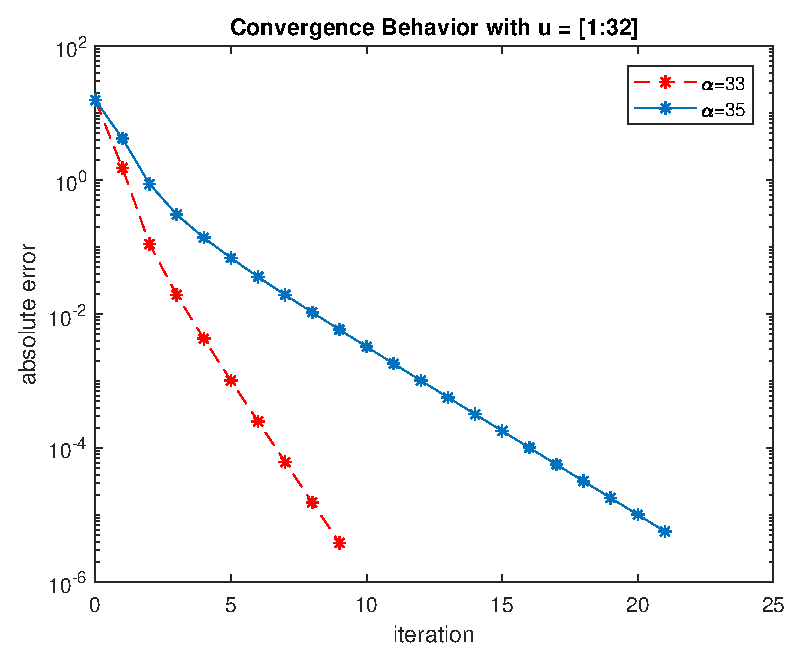
\includegraphics[width=\textwidth]{hw3p4p1.eps}
	\end{minipage}
	\hfill
	\begin{minipage}[b]{0.4\textwidth}
		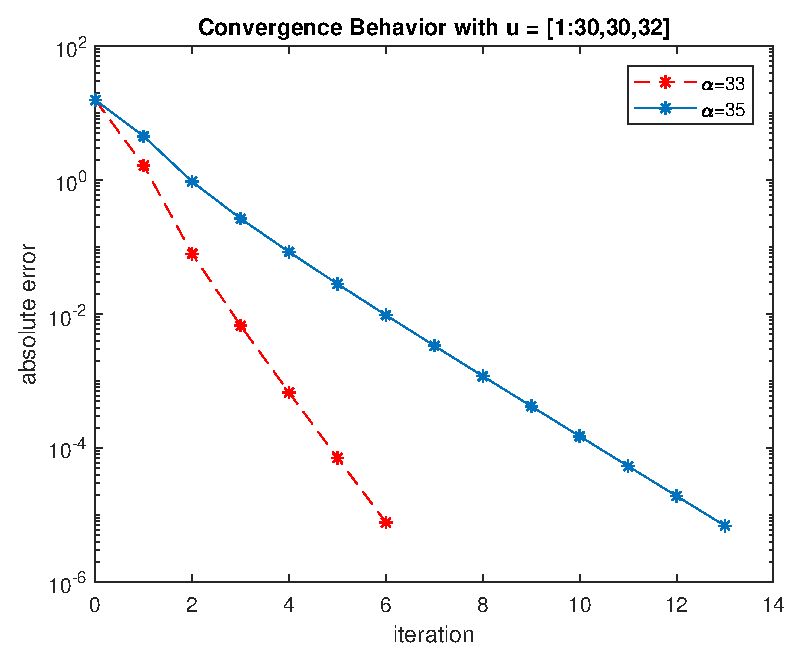
\includegraphics[width=\textwidth]{hw3p4p2.eps}
	\end{minipage}
\end{figure}
When we instead use the matrix $ A^* $ in our algorithm, we receive the plots
\begin{figure}[H]
	\centering
	\begin{minipage}[b]{0.4\textwidth}
		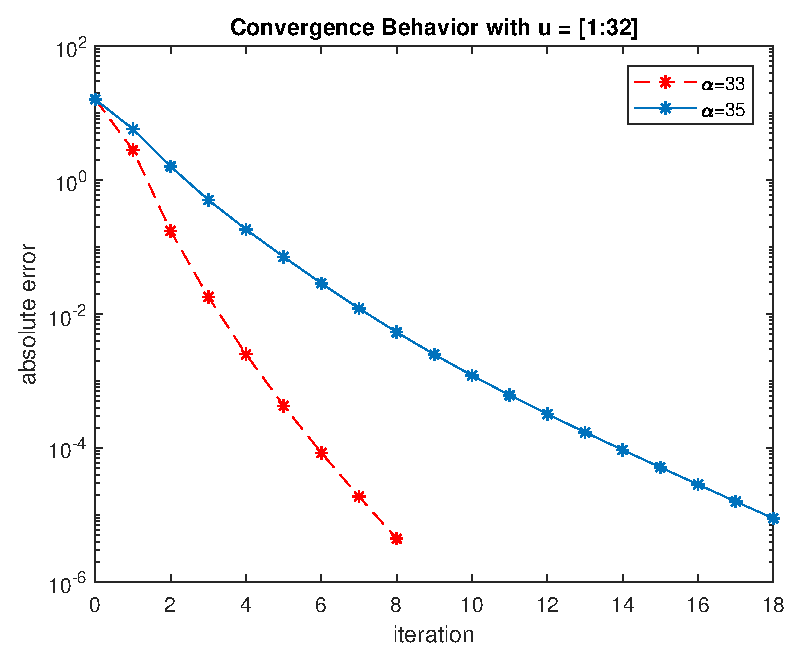
\includegraphics[width=\textwidth]{hw3p4p3.eps}
	\end{minipage}
	\hfill
	\begin{minipage}[b]{0.4\textwidth}
		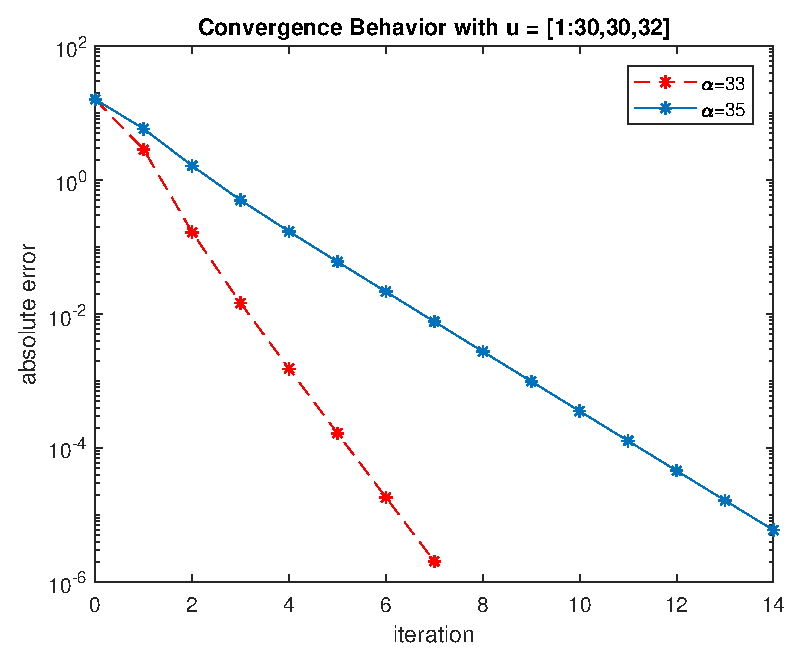
\includegraphics[width=\textwidth]{hw3p4p4.eps}
	\end{minipage}
\end{figure}
We see here that the convergence behavior is of the same order and has similar shape. Since $ A^* $ is simply a product of $ A $ with an orthonormal matrix and its inverse, the conditioning is the same. 

\bigbreak
%%%%%%%%%%%%%%%%%%%%%%%%%%%%%%%%%%%%%%%%%%%%%%%%%%%%%%%%%%%%%%%%%%%%%%%%%%%%%%%%%%%%%%%%%%%%%%%%%%%%

\problem{10} In this question we will play with two pictures (see Figure 8.9) that can be found in MATLAB's repository of images and can be retrieved by entering \texttt{load mandrill} and \texttt{load durer}. After loading these files, enter for each the command \texttt{colormap(gray)} and then \texttt{image(X)}. As you can see, these pictures feature the handsome mandrill and a drawing by the artist Albrecht D\"urer, who lived in the 1500s.
\begin{enumerate}[leftmargin=0.6cm,label=(\alph*)]
	\item Write a short MATLAB script for computing the truncated SVD of these images. For both pictures, start with rank $ r = 2 $ and go up by powers of 2, to $ r = 64 $. For a compact presentation of your figures use the command \texttt{subplot} for each of the pictures, with 3 and 2 as the first two arguments. (Check out \texttt{help subplot} for more information.)
	\item Comment on the performance of the truncated SVD for each of the pictures. State how much storage is required as a function of $ r $ and how much storage is required for the original pictures. Explain the difference in the effectiveness of the technique for the two images for small $ r $. [Use grayscale for calculations.]
\end{enumerate}

\vspace{-2 ex} \solution
\begin{enumerate}[leftmargin=0.6cm,label=(\alph*)]
	\item Our original image of the mandrill gives us
	\begin{figure}[H]
		\begin{center}
			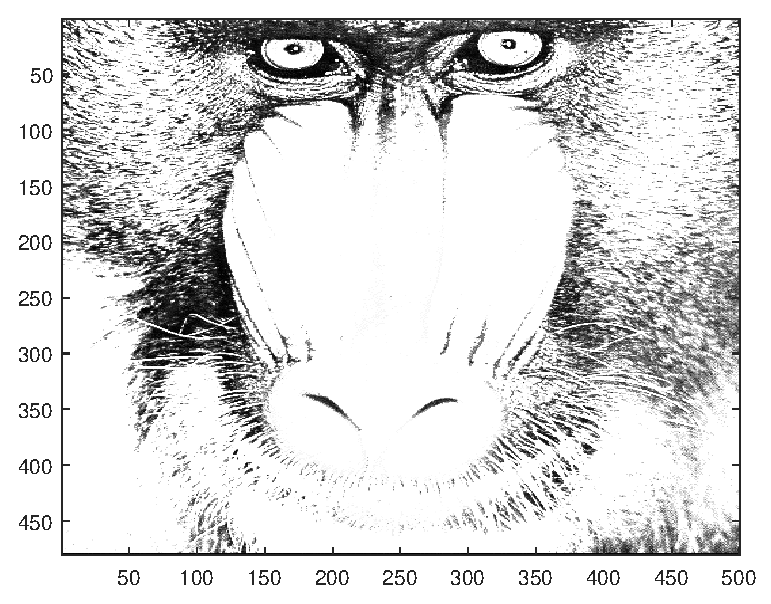
\includegraphics[scale=.6]{hw3p10p1.eps}
		\end{center}
	\end{figure}
	When we apply our different $ r $ values, we receive
	\begin{figure}[H]
		\begin{center}
			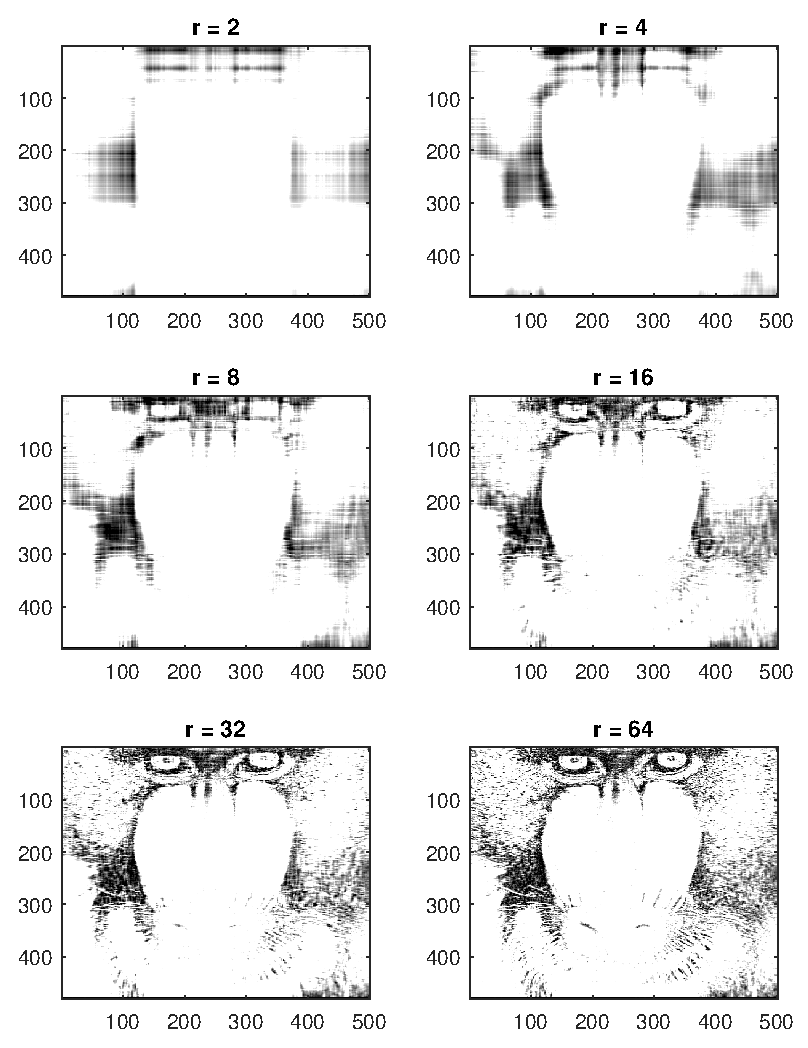
\includegraphics[scale=.8]{hw3p10p2.eps}
		\end{center}
	\end{figure}
	Our original image of the drawing by D\"urer gives us
	\begin{figure}[H]
		\begin{center}
			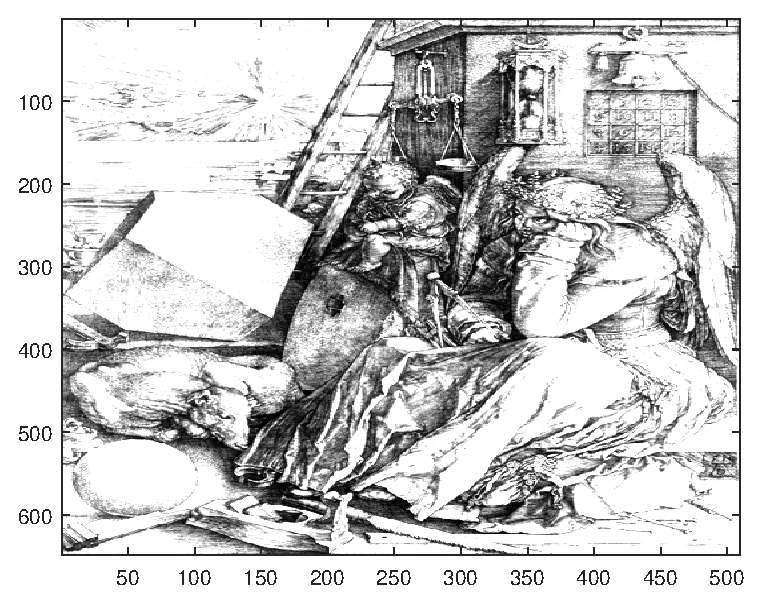
\includegraphics[scale=.6]{hw3p10p3.eps}
		\end{center}
	\end{figure}
	When we apply our different $ r $ values, we receive
	\begin{figure}[H]
		\begin{center}
			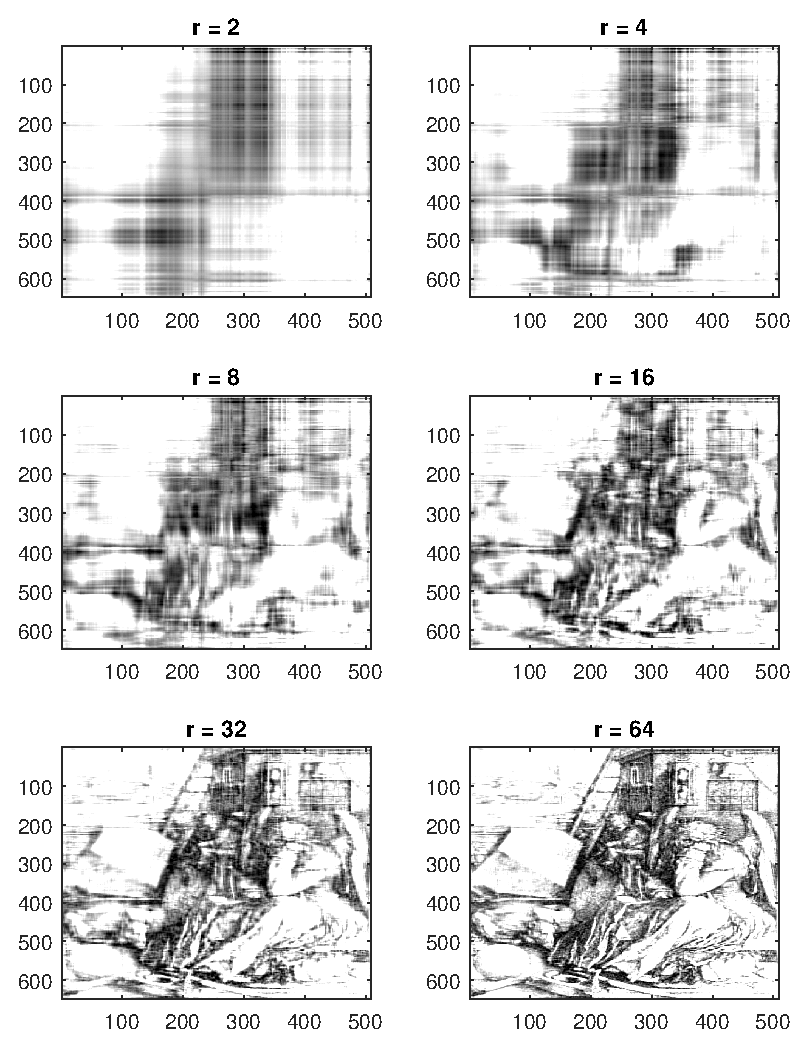
\includegraphics[scale=.8]{hw3p10p4.eps}
		\end{center}
	\end{figure}
	\item We see that the drawing by D\"urer starts to see faster changes as $ r $ increases. For the best $ r $ rank approximation of an $ m \times n $ matrix $ A $, we use
	\begin{align*}
	A_r = \sum_{i=1}^r \sigma_iu_iv_i^T
	\end{align*}
	where $ u_j $ is the $ j $-th column of $ U $, $ v_j^T $ is the $ j $-th row of $ V^T $, and $ \sigma_j $ is the $ j $-th singular value. This means that the amount of storage required is $ (m+n+1)r $, since each $ u_j $ vector is length $ m $, each $ v_j $ vector is length $ n $, and each singular value is length 1. Since the mandrill image has such a sharp gradient between features in the face, there are very few subtle features that are filled in for the middle values $ r $ values. Since there is a wider variation of shading in the D\"urer, we see finer features being filled in more rapidly. 
\end{enumerate}

{\hspace{-4 ex} \large \textbf{Appendix - Code listings}}\bigbreak

\large{Problem 10}
\begin{lstlisting}
clear all
close all
clc

colormap(gray)
load mandrill
figure(1)
image(X);

%%

[U,S,V] = svd(X);
figure(2)

subplot(3,2,1)
r1 = 2;
colormap(gray)
image(U(:,1:r1)*S(1:r1,1:r1)*V(:,1:r1)');
title('r = 2')

subplot(3,2,2)
r2 = 4;
colormap(gray)
image(U(:,1:r2)*S(1:r2,1:r2)*V(:,1:r2)');
title('r = 4')

subplot(3,2,3)
r3 = 8;
colormap(gray)
image(U(:,1:r3)*S(1:r3,1:r3)*V(:,1:r3)');
title('r = 8')

subplot(3,2,4)
r4 = 16;
colormap(gray)
image(U(:,1:r4)*S(1:r4,1:r4)*V(:,1:r4)');
title('r = 16')

subplot(3,2,5)
r5 = 32;
colormap(gray)
image(U(:,1:r5)*S(1:r5,1:r5)*V(:,1:r5)');
title('r = 32')

subplot(3,2,6)
r6 = 64;
colormap(gray)
image(U(:,1:r6)*S(1:r6,1:r6)*V(:,1:r6)');
title('r = 64')

%%

figure
load durer
colormap(gray)
image(X)

%%

[U,S,V] = svd(X);
figure(2)

subplot(3,2,1)
r1 = 2;
colormap(gray)
image(U(:,1:r1)*S(1:r1,1:r1)*V(:,1:r1)');
title('r = 2')

subplot(3,2,2)
r2 = 4;
colormap(gray)
image(U(:,1:r2)*S(1:r2,1:r2)*V(:,1:r2)');
title('r = 4')
subplot(3,2,3)

r3 = 8;
colormap(gray)
image(U(:,1:r3)*S(1:r3,1:r3)*V(:,1:r3)');
title('r = 8')

subplot(3,2,4)
r4 = 16;
colormap(gray)
image(U(:,1:r4)*S(1:r4,1:r4)*V(:,1:r4)');
title('r = 16')

subplot(3,2,5)
r5 = 32;
colormap(gray)
image(U(:,1:r5)*S(1:r5,1:r5)*V(:,1:r5)');
title('r = 32')

subplot(3,2,6)
r6 = 64;
colormap(gray)
image(U(:,1:r6)*S(1:r6,1:r6)*V(:,1:r6)');
title('r = 64')
\end{lstlisting}

\bigbreak
\large{Problem 4}
\begin{lstlisting}
% u = [1:32] example with no Q multiplication
clear all
close all
clc

u = 1:32;
A = diag(u);
I = eye(32);

A1 = A-33*I; A2 = A-35*I;

x = ones(32,1); x = x/norm(x);
initial = x'*A*x;

for i = 1:1000, 
	x = A1\x; x = x/norm(x); 
	lamA1(i) = x'*A*x; 
	if abs(lamA1(i)-32)<1e-5 break, end
end

x = ones(32,1); x = x/norm(x);

for i = 1:100, 
	x = A2\x; x = x/norm(x); 
	lamA2(i) = x'*A*x; 
	if abs(lamA2(i)-32)<1e-5 break, end
end


lamA1 = [initial lamA1];
semilogy(0:length(lamA1)-1,abs(lamA1-32),'r--*')
hold on
lamA2=[initial lamA2];
semilogy(0:length(lamA2)-1,abs(lamA2-32),'-*')

legend('\alpha=33','\alpha=35')
xlabel('iteration')
ylabel('absolute error')
title('Convergence Behavior with u = [1:32]')

%%

% u = [1:30,30,32] example with no Q multiplication
clear all
close all
clc

u = [1:30,30,32];
A = diag(u);
I = eye(32);

A1 = A-33*I; A2 = A-35*I;

x = ones(32,1); x = x/norm(x);
initial = x'*A*x;
for i = 1:1000, 
	x = A1\x; x = x/norm(x); 
	lamA1(i) = x'*A*x; 
	if abs(lamA1(i)-32)<1e-5 break, end
end

x = ones(32,1); x = x/norm(x);
for i = 1:100, 
	x = A2\x; x = x/norm(x); 
	lamA2(i) = x'*A*x; 
	if abs(lamA2(i)-32)<1e-5 break, end
end

lamA1 = [initial lamA1];
semilogy(0:length(lamA1)-1,abs(lamA1-32),'r--*')
hold on
lamA2=[initial lamA2];
semilogy(0:length(lamA2)-1,abs(lamA2-32),'-*')

legend('\alpha=33','\alpha=35')
xlabel('iteration')
ylabel('absolute error')
title('Convergence Behavior with u = [1:30,30,32]')

%%

% u = [1:32] example with Q multiplication
clear all
close all
clc


u = 1:32;
M = randn(32,32);
[Q,R] = qr(M);
A = Q*diag(u)*Q'; 
I = eye(32);

A1 = A-33*I; A2 = A-35*I;
x = ones(32,1); x = x/norm(x);
initial = x'*A*x;

for i = 1:1000, 
	x = A1\x; x = x/norm(x); 
	lamA1(i) = x'*A*x; 
	if abs(lamA1(i)-32)<1e-5 break, end
end

x = ones(32,1); x = x/norm(x);
for i = 1:100, 
	x = A2\x; x = x/norm(x); 
	lamA2(i) = x'*A*x; 
	if abs(lamA2(i)-32)<1e-5 break, end
end

lamA1 = [initial lamA1];
semilogy(0:length(lamA1)-1,abs(lamA1-32),'r--*')
hold on
lamA2=[initial lamA2];
semilogy(0:length(lamA2)-1,abs(lamA2-32),'-*')

legend('\alpha=33','\alpha=35')
xlabel('iteration')
ylabel('absolute error')
title('Convergence Behavior with u = [1:32]')

%%

% u = [1:30,30,32] example with Q multiplication

clearvars -except M 

close all

clc 


u = [1:30,30,32];

[Q,R] = qr(M);

A = Q*diag(u)*Q'; 

I = eye(32);


A1 = A-33*I; A2 = A-35*I;


x = ones(32,1); x = x/norm(x);

initial = x'*A*x;


for i = 1:1000, 

	x = A1\x; x = x/norm(x); 
	
	lamA1(i) = x'*A*x; 
	
	if abs(lamA1(i)-32)<1e-5 break, end

end


x = ones(32,1); x = x/norm(x);


for i = 1:100, 

x = A2\x; x = x/norm(x); 

lamA2(i) = x'*A*x; 

if abs(lamA2(i)-32)<1e-5 break, end

end


lamA1 = [initial lamA1];

semilogy(0:length(lamA1)-1,abs(lamA1-32),'r--*')

hold on

lamA2=[initial lamA2];

semilogy(0:length(lamA2)-1,abs(lamA2-32),'-*')


legend('\alpha=33','\alpha=35')

xlabel('iteration')

ylabel('absolute error')

title('Convergence Behavior with u = [1:30,30,32]')
\end{lstlisting}

\end{document}
